\chapter{Results}
This chapter evaluates the empirical performance of DKBRL and DKBSF.
It does this by comparing their performances with those of KBRL and KBSF
on the benchmark RL problems Mountain-Car, Acrobot, and Pinball.

\section{Experiment Design}
This section describes the way experiments were set up so anyone may
critique the methods or attempt to reproduce the results.
Since it would be impractical to enumerate all the relevant implementation
details, only the critically important points are mentioned.

\begin{description}

\item[Sampling Strategy]
I wanted to generate sample transitions whose start points 
uniformly cover the reachable part of the state space.
To generate reachable points,
I performed a random walk (selecting actions u.a.r. on every step) for $\approx10^6$
steps, starting from the start state and restarting whenever I reached the goal.
After generating these points, I subsampled the desired number of evenly spaced
points by clustering the points and taking the median of each cluster.

To reduce the correlation across datasets, I performed a separate random walk
for every time I needed a dataset.
Despite this, there is still correlation because the process of sampling for
coverage creates similar datasets.
Note that the sample transitions for the different actions all share the same set of
starts.
The plots that show ``number of samples'' below are all discussing the
number of sample transitions \textit{per action}.

\item[Domain Implementation]
My implementations of the three domains were each adapted from their
publicly available sources with some modifications.
First, I rescaled the domains to fill a unit cell.
Second, I refactored them to conform to my MDP solver's API.\footnote{
This mainly consisted of making the MDP instances immutable and renaming some
methods.}
Finally, I ended episodes where the agent failed to reach the goal after some 
number of steps $n_c$ ($500$ for Mountain-Car and Pinball, $1000$ for Acrobot).
When calculating average finishing time,
I treated the episodes where the agent failed to reach the goal as if the agent
reached the goal in $n_c$ steps.

\item[Learner Implementation]
I used my own implementations of KBRL and KBSF.
I implemented them as they were described in the papers introducing them
with three necessary modifications:
I implementated them to take a distance function as input and use that in
place of Euclidean distance for all kernel computations;
I modified KBRL so that the finite model it creates enforces the constraint
that terminal states self-transition with zero reward;
in the event of arithmetic underflow when performing local averaging,
I automatically take the value predicted by the nearest neighbour.

I used a Gaussian as my mother kernel in all experiments.
For the parts involving linear algebra, I used the matrix libraries
EJML\footnote{https://code.google.com/p/efficient-java-matrix-library/} and
Parallel Colt.\footnote{
https://sites.google.com/site/piotrwendykier/software/parallelcolt}

For DKBRL and DKBSF, I do not resample between iterations even though this
is necessary for maintaining the correctness guarantees of KBRL (as noted in
the previous chapter).
I decided against resampling because the added computational cost would
outweigh the potential improvement in solution quality.

\item[Parameters]
The purpose of these experiments is to demonstrate typical case performance,
not to show what happens with optimally chosen settings.
As a result I did not attempt to tune any parameters.
For most of these parameters, the value chosen affects KBRL/KBSF and
DKBRL/DKBSF identically.

For the bandwidths, I picked a range of bandwidths I expected would be
representative based my experiences when implementing the algorithms.
For $\alpha$, I chose $1$ in every test (except where stated otherwise) because
it was consistently adequate in the tests I performed for Chapter 4.
I capped the number of iterations of DKBRL at four; the experiments in
Chapter 4 suggest this would be sufficient.
For the sustained actions, I chose $\epsilon=.1$ ($0.15$ for Acrobot),
a number within an order of magnitude of the expected minimum distance between
points for sample densities used.
\end{description}
That covers all the important details about the experiment design.
We now proceed to the results.

\section{Mountain-Car}
Mountain-Car is a two dimensional MDP described by Sutton and Barto
\cite{rlai}.
The code was adapted from RL-Glue \cite{rlglue} .
Mountain-Car is meant to simulate a car with a weak motor attempting to
drive out of a valley.
The car is not powerful enough to escape directly and must build up
energy by swing back and forth.
The two dimensions correspond to the car's position and its velocity.
The car has three actions: REVERSE, NEUTRAL, and FORWARD.
The optimal trajectory out of the valley is 102 steps long.

\begin{figure}[!!!ht]
  \centering
    \includegraphics[width=90mm]{figs/mcexpl.png}
  \caption[Mountain-Car domain]{Picture of the Mountain-Car domain
(taken from rl-community.org, available under GNU Free Documentation Licence)}
\end{figure}

Despite its simplicity, Mountain-Car is an interesting domain that
illustrates some key properties of DKBRL.
Mountain-Car's value function has a discontinuity that spirals through the
state space (See Figure 5-2).
This spiral separates points where the car has enough energy to make it up
the hill on its current swing from points where the car needs to make an
extra swing.
The spiral occurs in slightly different positions in the Q-Values of the three
actions.
A good transform is one that unrolls the space along the spiral.

\begin{figure}[!htb]
  \minipage{0.5\textwidth}
    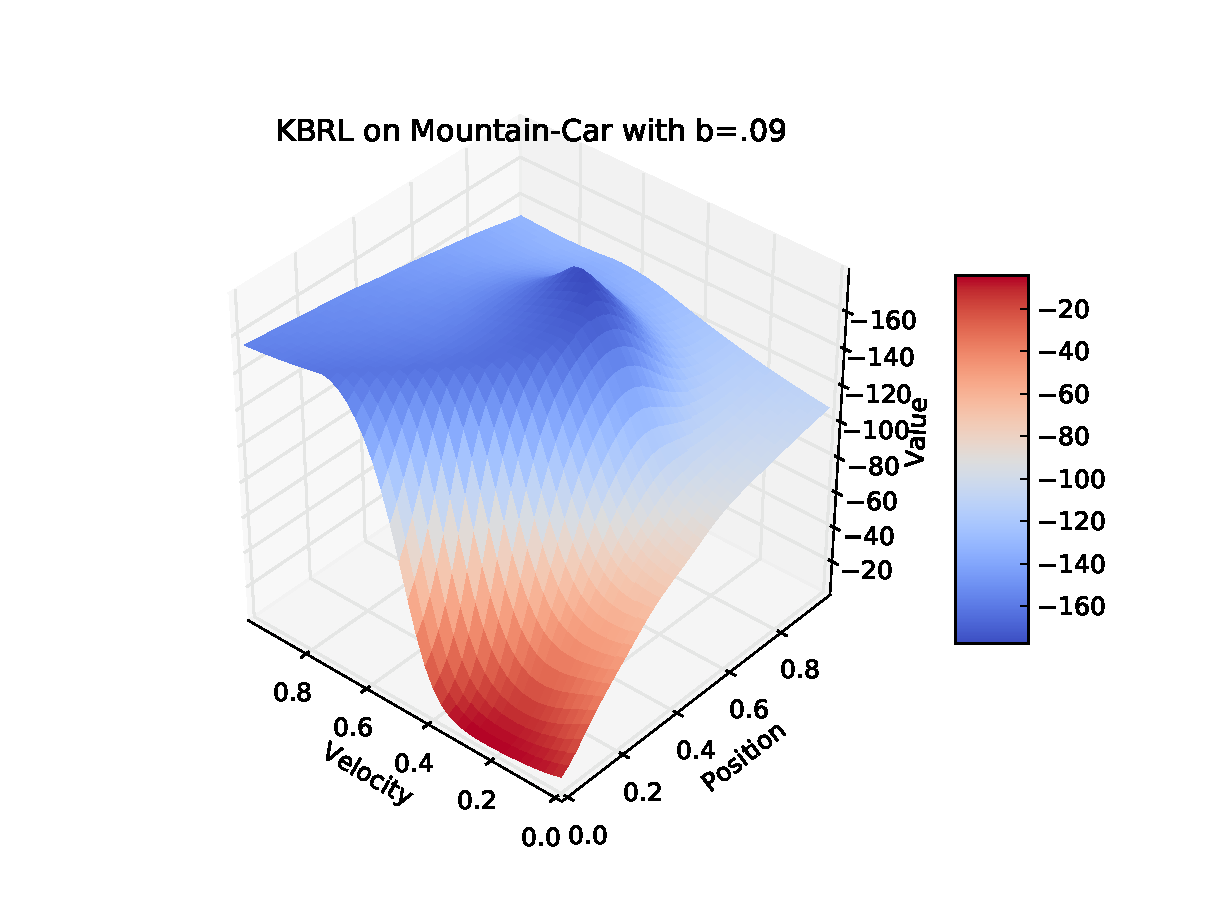
\includegraphics[width=\linewidth]{figs/chap5/mc09first.pdf}
  \endminipage\hfill
  \minipage{0.5\textwidth}
    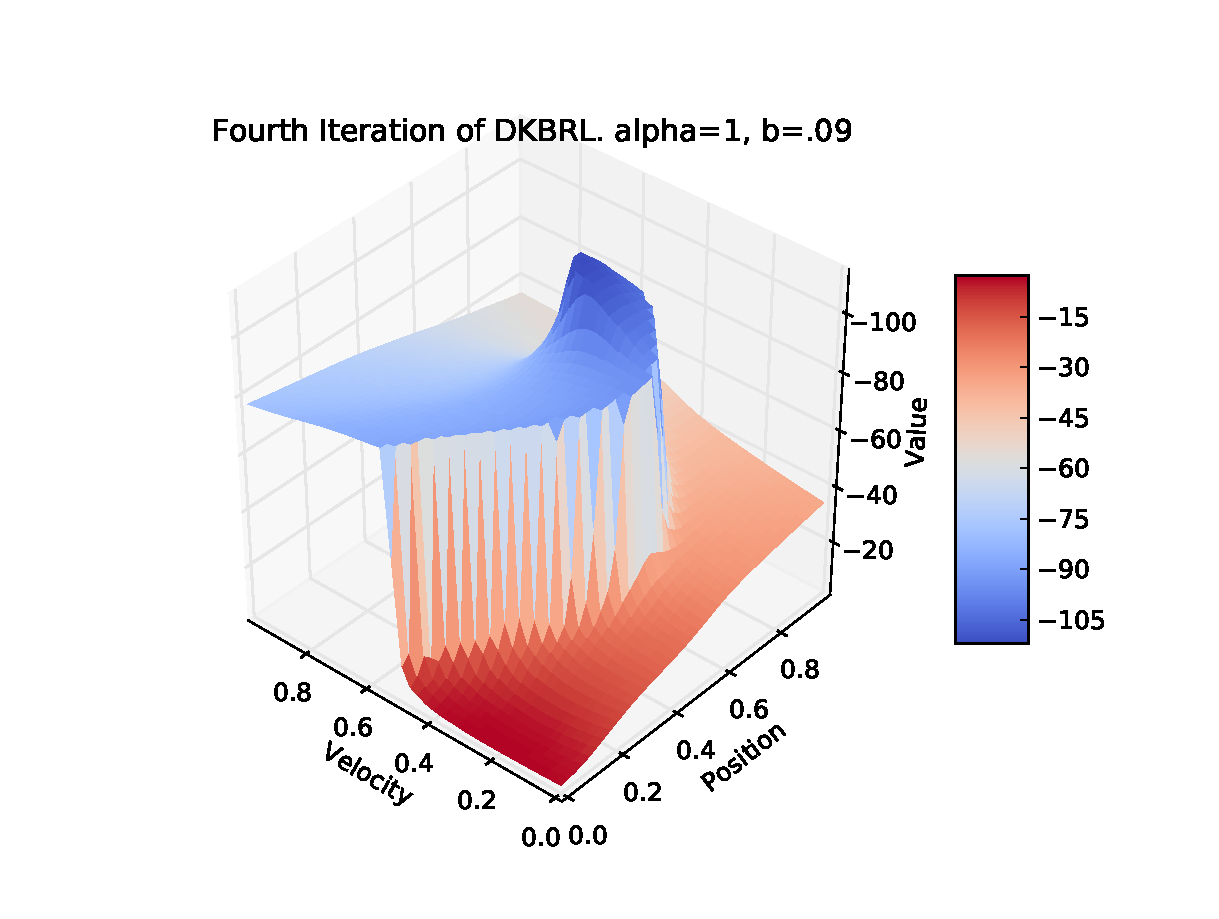
\includegraphics[width=\linewidth]{figs/chap5/mc09fourth.pdf}
  \endminipage
\caption[DKBRL approximation of Mountain-Car value function]
{On the left, Mountain-Car's value function as represented by KBRL.
On the right, Mountain-Car's value function after four iterations of DKBRL.
Both were made with the same set of transitions and a bandwidth of $.09$.
Note at how well DKBRL captures the discontinuity.
Also note the axes; the value DKBRL finds for the bottom of the hill
is closer to the true value of $-102$.}
\end{figure}

DKBRL is able to fit the value function well across a range of
bandwidths and sample sizes.
To see how this translates to solution quality I ran two types of experiments,
one holding the number of samples fixed and varying the bandwidth and
the other holding the bandwidth fixed and varying the number of samples.

\begin{figure}[!!!ht]
  \centering
    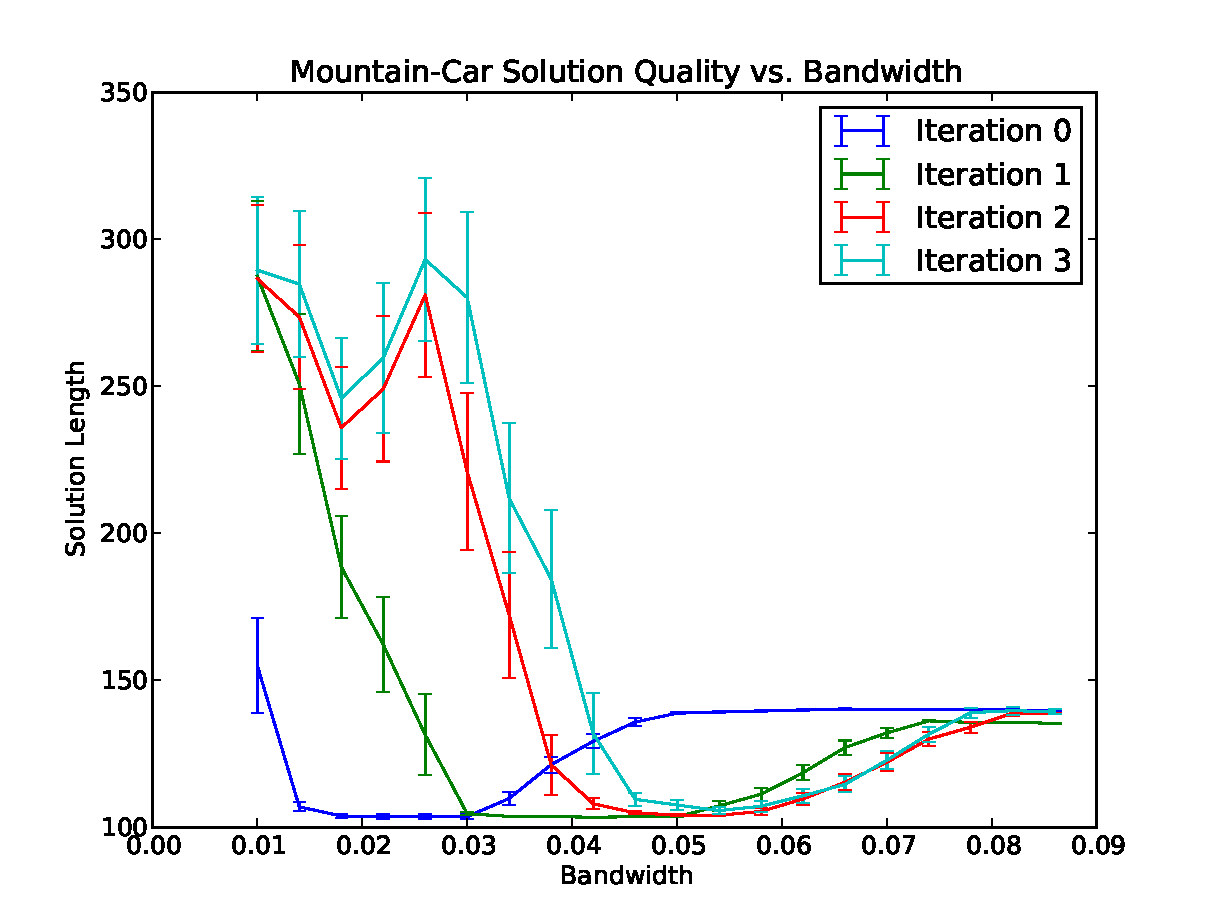
\includegraphics[width=90mm]{figs/chap5/mcband.pdf}
  \caption[Mountain-Car bandwidth sensitivity on each iteration of DKBRL]
{The average solution trajectory length on every iteration of
DKBRL. KBRL is equivalent to Iteration 0. The final solution returned by
DKBRL is the lower envelope of all the curves.}
\end{figure}

Figure 5-3 shows the sensitivity of the solution quality to the bandwidth
holding the sample size fixed at 600 transitions per action.
The graph shows the solution quality averaged over 40 trials.
Solution quality is measured as the length of the trajectory from start to
goal.
The error bars correspond to  one standard error.

Let us examine the features of this graph.
First note that KBRL (which corresponds to iteration 0)
is able to find the optimal solution when the bandwidth is in the
$.015$--$.03$ range. 
For these bandwidths, transforming makes the solution worse.
For larger bandwidths, FIIRA makes the solution better.
Note that there is a large difference in the curves for iteration 0 and
iteration 1.
This suggests that the setting $\alpha = 1$ is too high for this domain.

DKBRL retains the best policy it finds over all its iterations.
Thus, the final solution returned by DKBRL corresponds to the lower envelope of all
the curves in Figure 5-3.
Figure 5-4 plots this agianst the KBRL solution (which is equivalent to
Iteration 0) to see the extent of the improvement.
Note how DKBRL almost triples the range of bandwidths for which it is possible
to find the optimal trajectory.
Also note that DKBRL finds the optimal trajectory with lower
variance.

\begin{figure}[!!!ht]
  \centering
  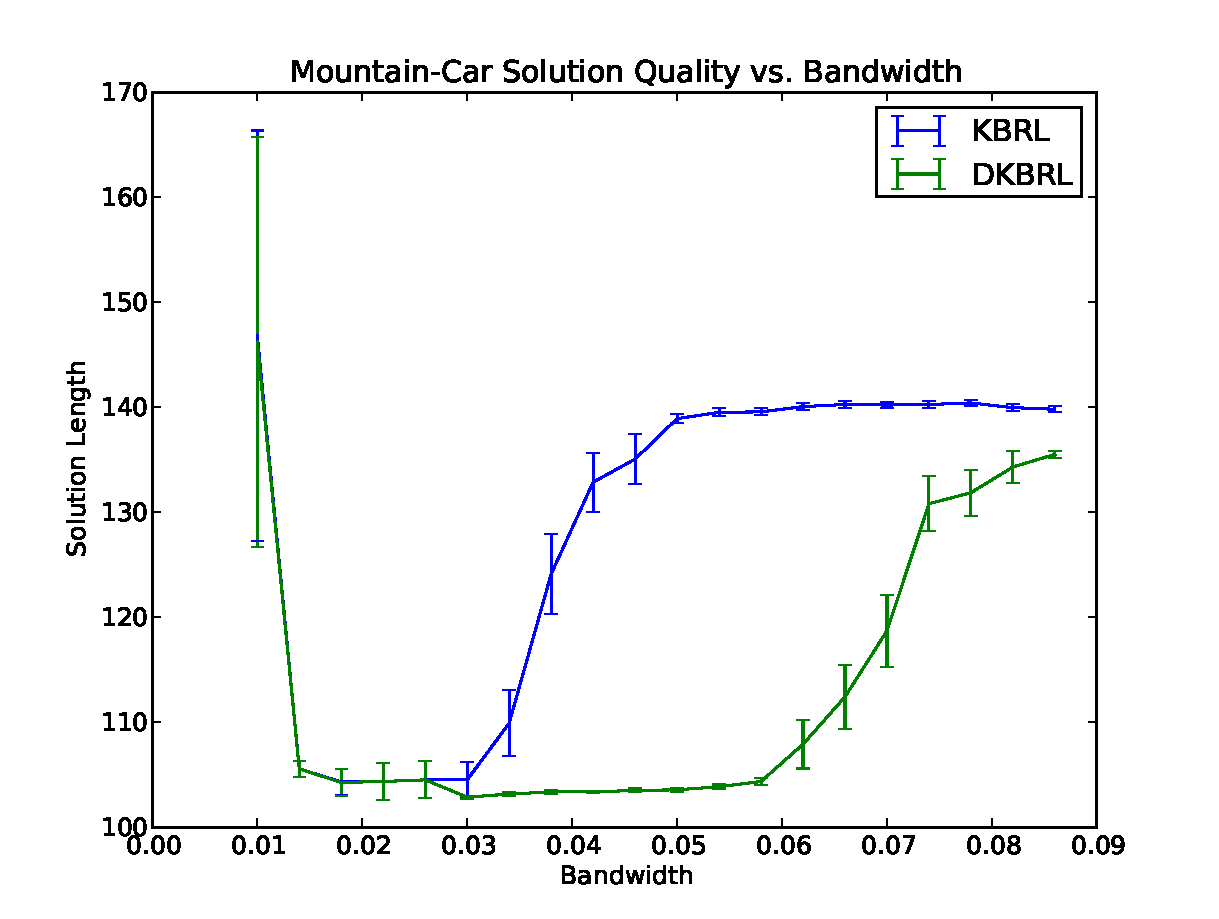
\includegraphics[width=90mm]{figs/chap5/mcband2.pdf}
  \caption[Bandwidth sensitivities of KBRL and DKBRL on Mountain-Car]
{The bandwidth sensitivities of KBRL and DKBRL on Mountain-Car.}
\end{figure}

The next three figures show the effect of sample size on solution quality
averaged over 20 trials for three different values of the bandwidth.
For small bandwidths, DKBRL is not able to improve upon KBRL.
For intermediate bandwidths, DKBRL greatly improves upon KBRL, which does not
manage to reach the optimal solution for any sample size.
On the other hand, given enough samples, DKBRL allows the agent to
consistently find the optimal solution.
Note that the DKBRL curve for $b=.05$ is slightly better than the
one for $b=.03$.
For large bandwidths, DKBRL improves on KBRL but does not find the optimal
solution consistently.
I conjecture that this is because we are approaching minimum
bandwidth needed to adequately model the dynamics of the system.

\begin{figure}[!!!ht]
  \centering
    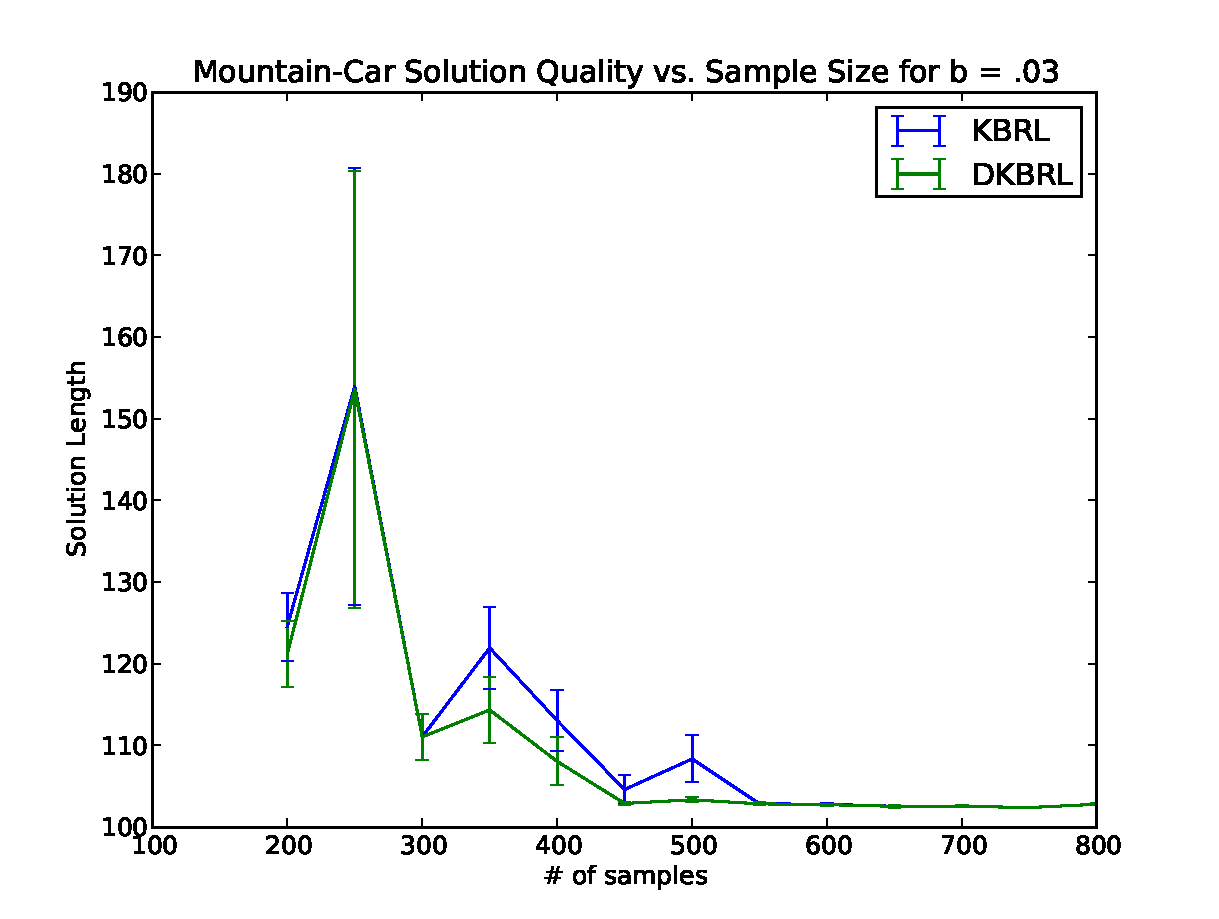
\includegraphics[width=75mm]{figs/chap5/mc03.pdf}
  \caption[KBRL vs. DKBRL with small bandwidth on Mountain-Car]
{DKBRL does not improve upon KBRL when the bandwidth is small.}
\end{figure}
\begin{figure}[!!!ht]
  \centering
    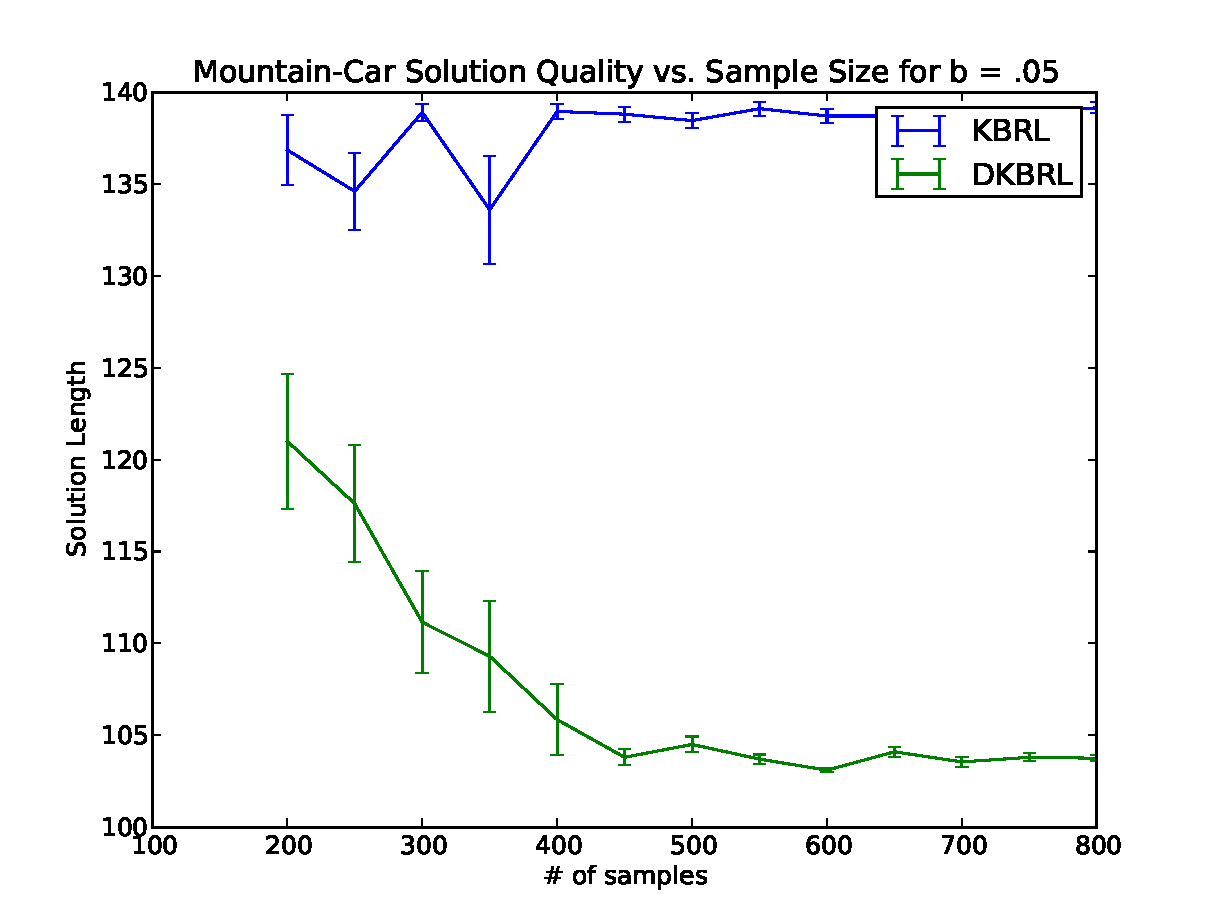
\includegraphics[width=75mm]{figs/chap5/mc05.pdf}
  \caption[KBRL vs. DKBRL with itermediate bandwidth on Mountain-Car]
  {DKBRL significantly improves upon KBRL when the bandwidth is
intermediate.}
\end{figure}
\begin{figure}[!!!ht]
  \centering
    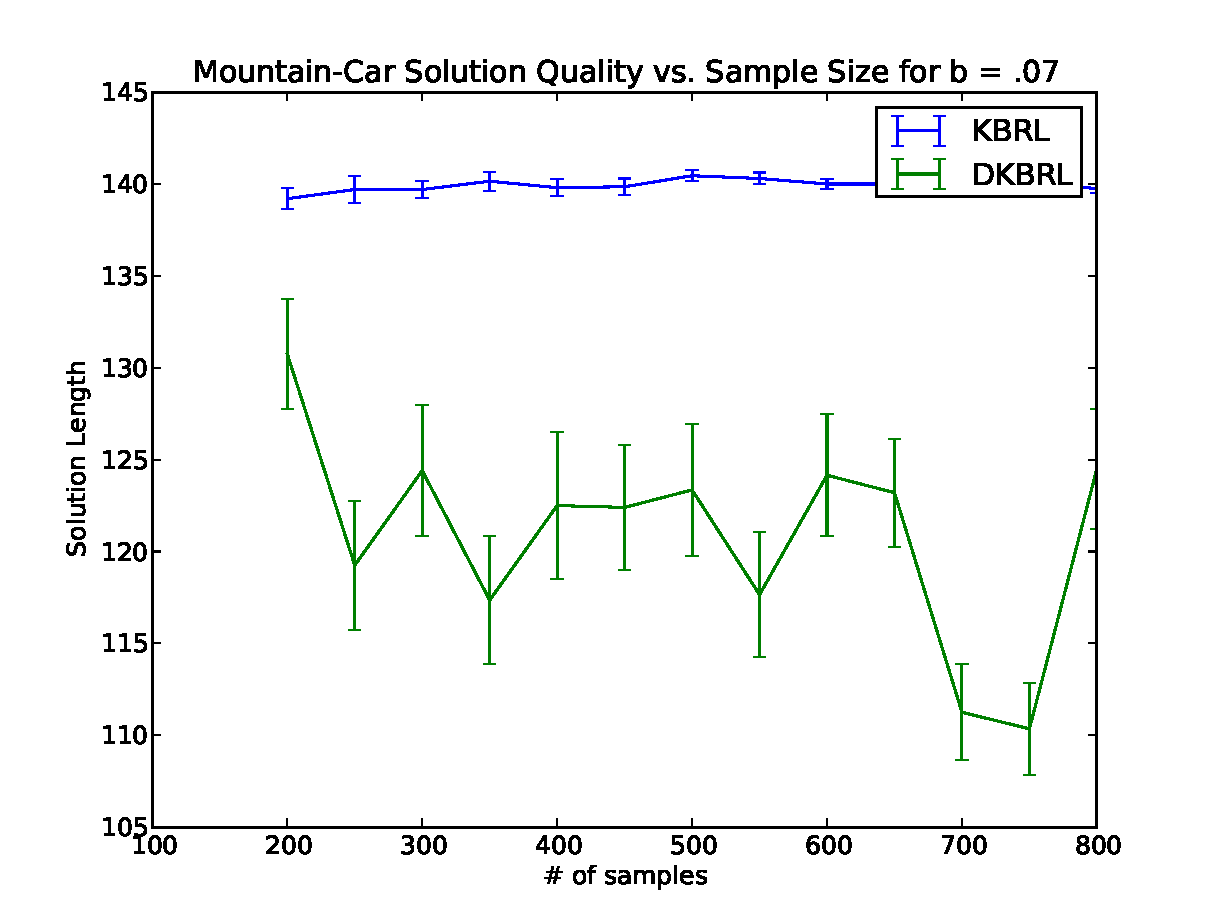
\includegraphics[width=75mm]{figs/chap5/mc07.pdf}
  \caption[KBRL vs. DKBRL with large bandwidth on Mountain-Car]
{DKBRL improves upon KBRL when the bandwidth is large, but not as
much as it does when the bandwidth is intermediate.}
\end{figure}

These experiments show that DKBRL is capable of improving upon the solution
generated by KBRL.
This improvement in the solution quality is not as large as the improvement in the
value function approximation.
This is because representing the value function well is not necessary for
solving Mountain-Car (or any MDP in general).
All that matters is that the best action gets assigned the highest Q-Value.
This means DKBRL might not produce a better policy even if it improves on
the value function approximation.
In fact, it can produce a worse policy if it changes the ranking of the actions
in the wrong direction.

\section{Acrobot}
Acrobot is a four dimensional MDP by Sutton and Barton \cite{rlai}.
It models a two-link, underactuated robot that is anchored at one end,
similar to a gymnast on a high bar.
The agent's objective is to get its leg above some height.

The four dimensions correspond to the angles and angular velocities of the two
links.
There are three discrete actions (LEFT, RIGHT, and IDLE) corresponding to
how the agent can actuate the joint between the two links.
The code I used was adapted from \cite{rlglue}
The best solution trajectory I observed during my experiments 112 steps long.

\begin{figure}[!!!ht]
  \centering
    \includegraphics[width=30mm]{figs/abexpl.png}
  \caption[Acrobot domain]{Picture of the Acrobot domain
(taken from rl-community.org, available under GNU FDL)}
\end{figure}

To evaluate DKBRL's performance on Acrobot, I repeated the experiments I did
on Mountain-Car.
In the first set of experiments, I set the number of samples fixed at 3000
transitions per action and varied the bandwidth.
The results (Figure 5-9) showed that the optimal number of iterations was
different at different bandwidths.
Iteration 0 (KBRL) does not appear to be optimal anywhere, though the error bars
are too large to be sure.

\begin{figure}[!!!ht]
  \centering
    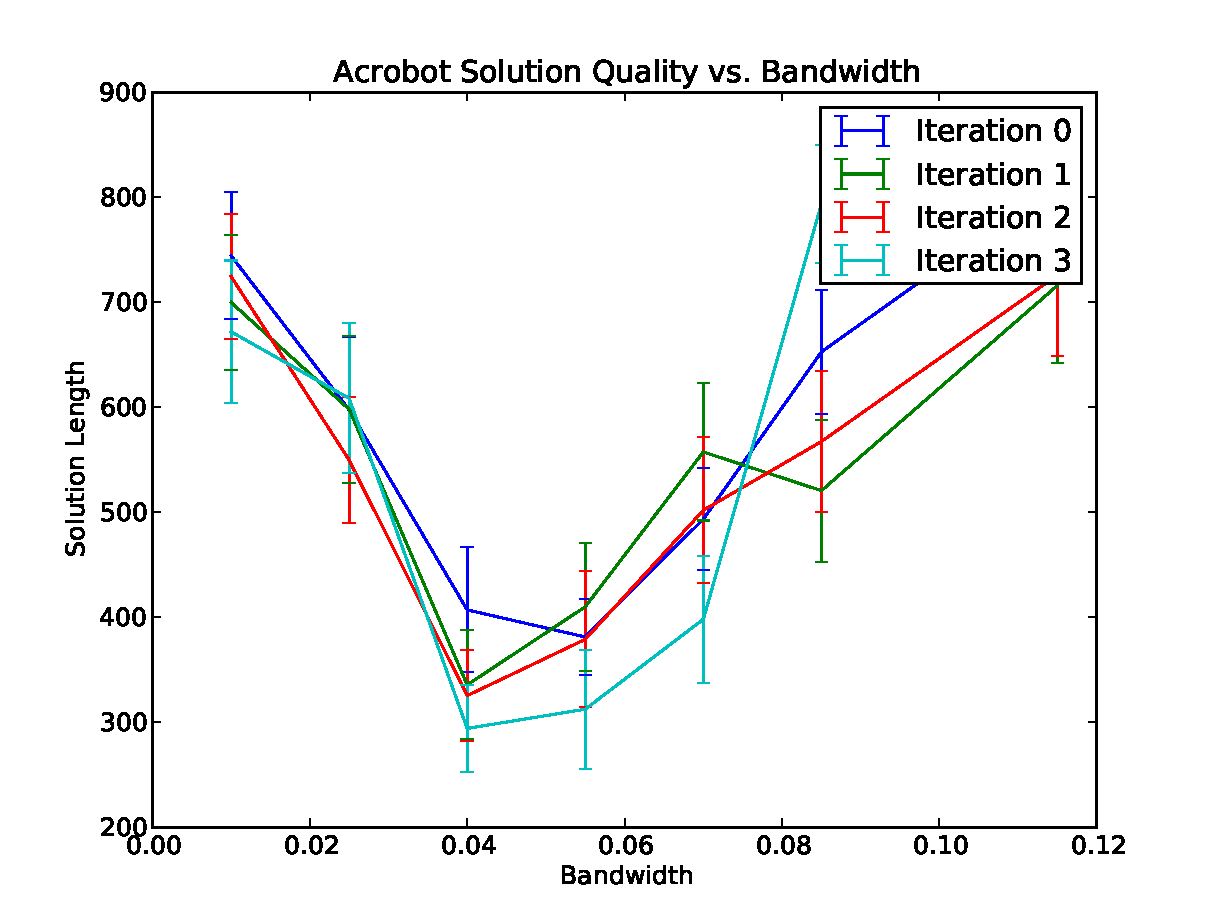
\includegraphics[width=90mm]{figs/chap5/acroband.pdf}
  \caption[Acrobot bandwidth sensitivity on each iteration of DKBRL]
{Solution quality vs. bandwidth over four iterations of DKBRL,
  averaged over 20 trails.}
\end{figure}

To see how DKBRL compares to KBRL, we can again plot the lower envelope of
all the iterations against Iteration 0. This is shown in Figure 5-10.
Note how DKBRL is able to find better solutions across all bandwidths.
Be aware that an average solution length of 900 does not mean the solver was
finding paths that were 900 steps long.
It means that in most episodes the agent could not reach the goal
(these are treated as 1000) and in three or four episodes the agent reached
the goal quickly.
This is why the standard errors are so high.

\begin{figure}[!!!ht]
  \centering
    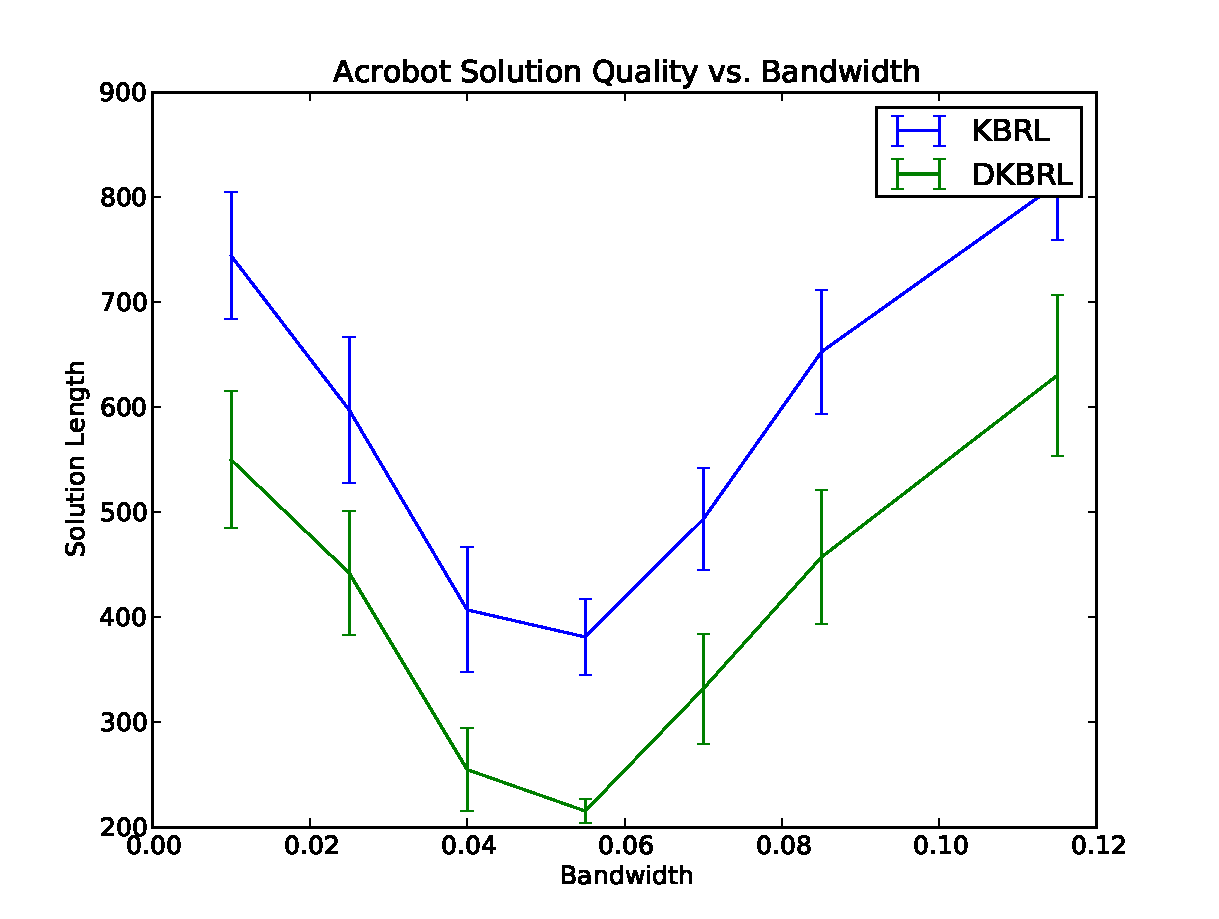
\includegraphics[width=90mm]{figs/chap5/acroband2.pdf}
  \caption[Bandwidth sensitivities of KBRL and DKBRL on Acrobot]
{The bandwidth sensitivities of KBRL and DKBRL on Acrobot.}
\end{figure}

The next set of experiments held the bandwidth fixed and varied the number of
samples.
The results of these are shown in Figure 5-11.
Note how DKBRL produces substantially better solutions for all sample size and bandwidth
combinations.
Still, DKBRL was not able to consistently find the optimal solution.

\begin{figure}[!htb]
  \minipage{0.33\textwidth}
    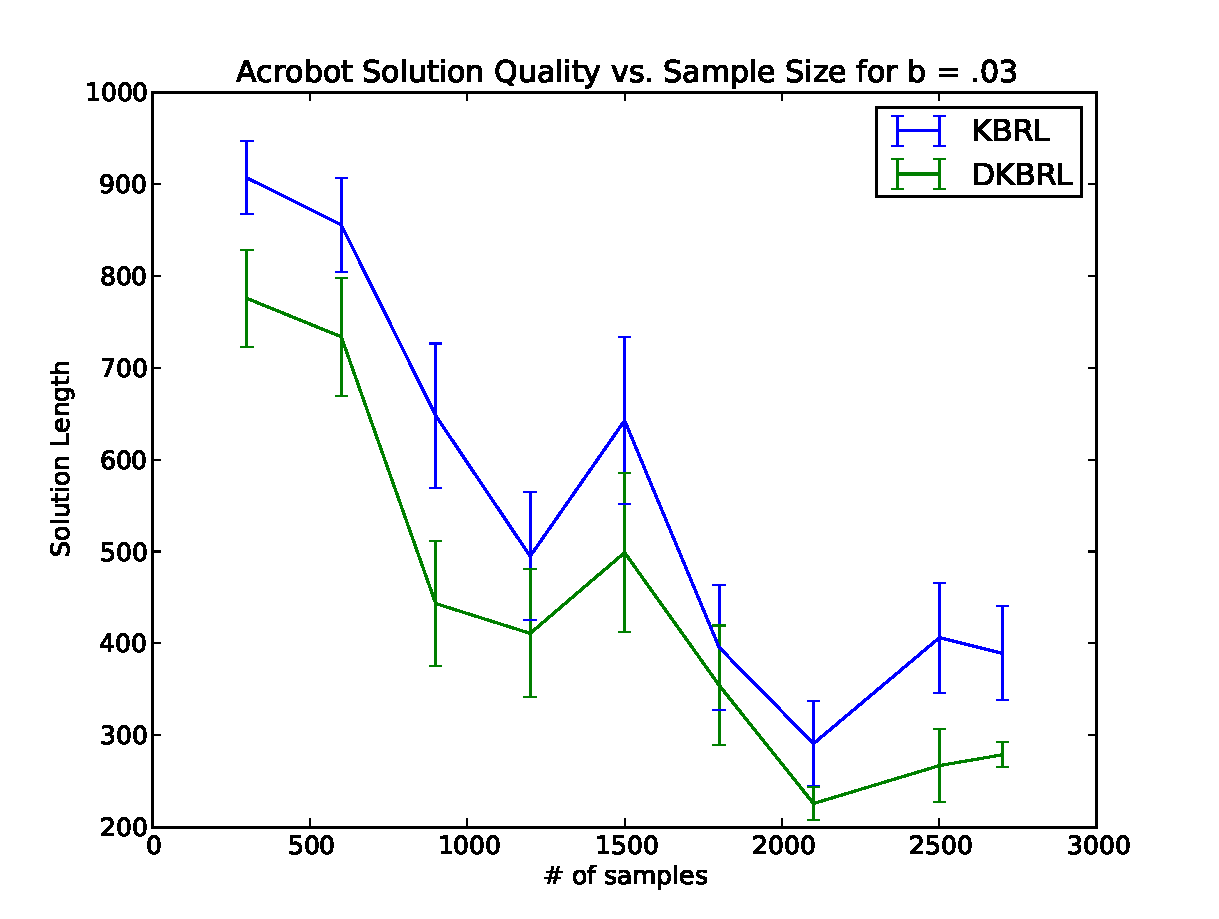
\includegraphics[width=\linewidth]{figs/chap5/acr03.pdf}
  \endminipage\hfill
  \minipage{0.33\textwidth}
    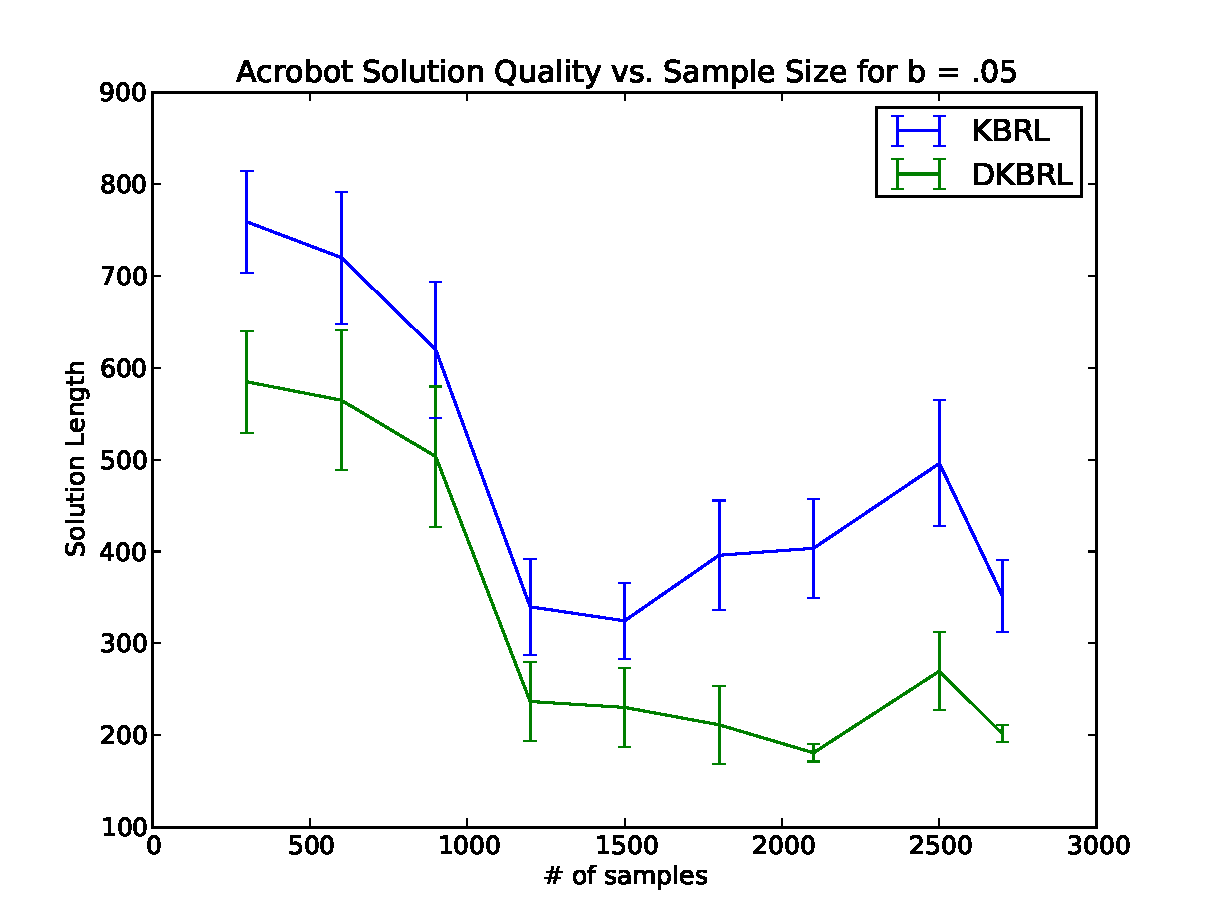
\includegraphics[width=\linewidth]{figs/chap5/acr05.pdf}
  \endminipage\hfill
  \minipage{0.33\textwidth}
    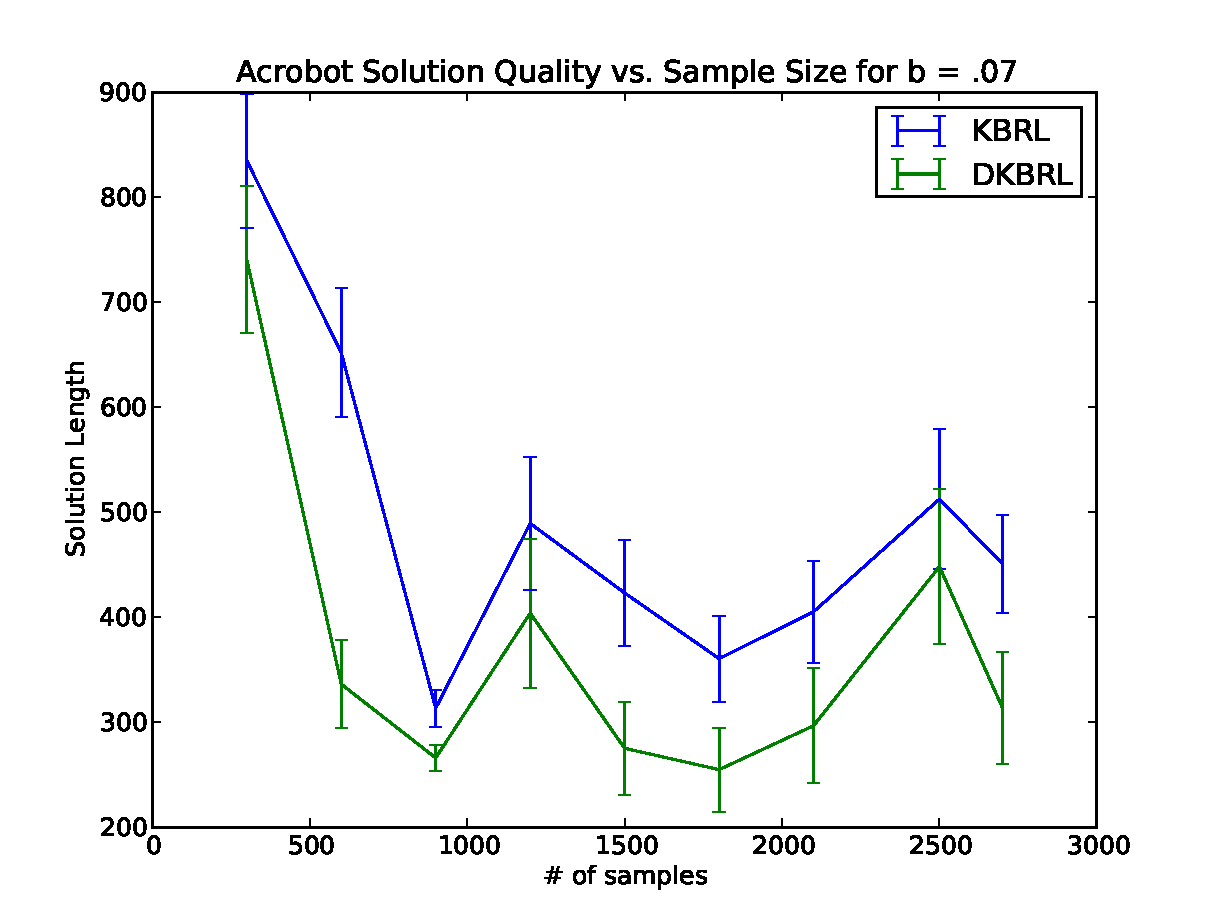
\includegraphics[width=\linewidth]{figs/chap5/acr07.pdf}
  \endminipage
\caption[KBRL vs. DKBRL on Acrobot]
{The solution qualities of KBRL and DKBRL for different bandwidths
and number of samples averaged over 20 trials.}
\end{figure}

These experiments showed that DKBRL is able to produce substantial improvements
in solution quality when performed on Acrobot.
This suggests that representing the value function correctly is more
important in Acrobot than in Mountain-Car.

\section{PinBall}
PinBall is an even more challenging 4D MDP described in \cite{gdk}.
In PinBall, the agent models a ball trying to navigate through a maze towards
a goal.
The agent has five actions, UP, DOWN, LEFT, RIGHT, and COAST.
The agent incurs a penalty when taking one of the first four actions.
To navigate efficently, the agent must bounce off the obstacles to change
direction without accelerating.

\begin{figure}[!!!ht]
  \centering
    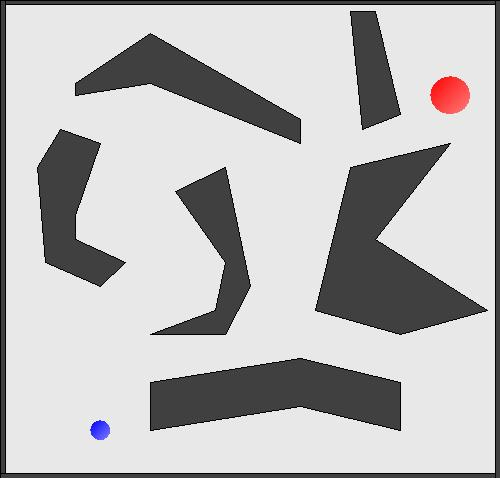
\includegraphics[width=60mm]{figs/chap5/pbeasy.jpg}
  \caption[PinBall domain map]{Map of the PinBall domain.
The start point is marked in blue and the end point in red.
(Picture taken from http://www-all.cs.umass.edu/~gdk/pinball/ with permission)}
\end{figure}

In PinBall, a random walk does not provide good coverage of the state space.
This is because the ball never builds up momentum and high velocity states do
not get reached.
To get around this, I sampled ball positions for reachability and velocities
at random.

PinBall is a challenging domain because the volume of the reachable state space
is much higher than that of Acrobot.
It is also filled with narrow corridors that are difficult to pass through
without a good policy.

PinBall is an especially interesting domain because, it allows for more
intricate transforms.
In PinBall, variation in velocity does not affect the value of a state nearly
as much as variation in position.
Two points with the same velocity but large difference in position will have
a greater difference in value that points with the same position and large
difference in velocity.
This means a good transform will squash the space along the velocity
dimensions.
This reduces the volume of the state space making the problem easier to solve.

Because PinBall is such a difficult domain, solving it non-parametrically is
extremely computation intensive.
As a result, I could not perform the same type of tests I did for Mountain-Car
and Acrobot. Instead I picked some settings of parameters and ran a few trials
of the algorithm.

For the first batch of tests I chose to use DKBSF.
Since Barreto et. al. \cite{kbsf} give no guidance on the optimal ratio of sample
transitions to representative points for a given amount of compute time,
I had to pick these arbitrarily.
I collected 30000 sample transitions per action and 5000 representative points 
and chose a bandwidth of .03 \footnote{The sample size was set by the amount of
memory available on the machine used for the experiments and the bandwidth was 
the smallest number that didn't result in arithmetic underflows when
evaluating the kernel}.
Each trial took roughly a day to perform.

\begin{table}[H]
\begin{center}
    \begin{tabular}{| l | l | l | l |}
    \hline
Trial & Alpha & Iter. 0 & Iter. 1 \\ \hline
0 & .16 & -- & 360\\
1 & .16 & -- & 230\\
2 & .25 & -- & 235\\
3 & .25 & -- & 245\\
4 & .16 & 157 & ERROR\\
5 & .16 & -- & --\\
6 & .16 & -- & --\\
7 & .16 & 252 & 176\\
8 & .16 & -- & 169\\
9 & .16 & -- & --\\
10 & .16 & -- & --\\
    \hline
    \end{tabular}
\end{center}
    \caption[DKBSF Pinball results]
{The number of steps to reach the goal in 11 trials of DKBSF on PinBall.
A ``--'' means the agent did not reach the goal.}
\end{table}

Table 5.1 shows the result of this experiment.
A ``--'' means the ball did not make it to the goal.
An ``ERROR'' means the program crashed mid computation\footnote{There was
supposed to be a column for Iteration 2 but it was full of ``ERROR''s and
is omitted.}.
As before, Iteration 0 is equivalent to KBSF and the subsequent iterations
show the improvement resulting from DKBSF.
From this table, it appears DKBSF is offering some advantage, though it is
not possible to say how much.
KBSF was only able to reach the goal in 2 out of 11 trials while DKBSF did so
in 6 out of 10.

\begin{figure}[!!!ht]
  \centering
    \includegraphics[width=90mm]{figs/apdx/f1.png}
  \caption[DKBSF on PinBall sample trajectory]{The trajectories generated
on trial 1. Iteration 0 (KBSF) is on the left and iteration 1 (DKBSF) is on
the right. The path is colored by time; a full cycle through the hues
corresponds to 100 steps.
Note how KBSF misses the narrow corridor then attempts to go through the wall
while DKBSF makes it through. The remaining trajectories are in the appendix. }
\end{figure}

For the next batch of experiments, I tried DKBRL with a sample size of
10000 transitions per action and a bandwidth of $.15$.
The results of that experiment are shown in Table 5.2.

\begin{table}[H]
\begin{center}
    \begin{tabular}{| l | l | l | l | l |}
    \hline
Exp\# & Alpha & Iter. 0 & Iter. 1 & Iter 2. \\ \hline
0 & 1 & -- & 243 & --\\
1 & 1 & -- & -- & --\\
2 & 1 & -- & -- & --\\
3 & 1 & -- & 356 & --\\
4 & 1 & -- & -- & --\\
5 & 1 & -- & 294 & --\\
6 & 1 & -- & 377 & --\\
7 & 1 & -- & 258 & --\\
8 & 1 & -- & 429 & --\\
9 & 1 & -- & 332 & --\\
10& 1 & 255 & 382 & --\\
    \hline
    \end{tabular}
\end{center}
    \caption[DKBRL PinBall results]{The results of running DKBRL on PinBall.}
\end{table}

The results of this experiment are similar to those for KBSF.
Using KBRL alone, the ball was only able to get the goal once out of eleven
trials; however, after a single iteration of DKBRL the ball made it on
eight trials.
Performing an additional iteration made the performance worse.\\

\begin{figure}[!!!ht]
  \centering
    \includegraphics[width=110mm]{figs/apdx/r0.png}
  \caption[DKBRL on PinBall sample trajectory]{The trajectories generated
on trial 0. KBSF attempts to go straight up,
iteration 1 of DKBSF goes around around all the obstacles,
iteration 2 gets stuck in a corner. Most of the trials looked very similar to this.}
\end{figure}

\begin{figure}[!!!ht]
  \centering
    \includegraphics[width=110mm]{figs/apdx/r10.png}
  \caption[DKBRL on PinBall sample trajectory 2]{The trajectories generated
on trial 10, the only trajectory where KBRL reached the goal.}
\end{figure}

Together, the experiments in this chapter show that FIIRA is capable of
offering tangible performance improvements when applied to KBRL.